\documentclass[tikz, border=5pt]{standalone}
\usepackage[dvipsnames]{xcolor}
\usetikzlibrary{patterns}

\begin{document}
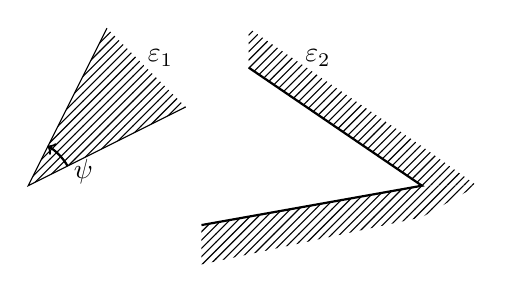
\begin{tikzpicture}

    %% Types of cones

    % Acute
    \begin{scope}
        \draw (1,2) -- (0,0) -- (2,1);
        \fill[pattern=north east lines] (1,2) -- (0,0) -- (2,1);
        \node[above right=-3] at (1.5,1.5) {\( \varepsilon_1 \)};
        \draw[->, thick] (2/4,1/4) arc[start angle=30, end angle=60, radius=0.7];
        \node[above=5, right=13] at (0,0) {\( \psi \)};
    \end{scope}

    % Obtuse
    \begin{scope}[xshift=5cm]
        \draw[thick] (-2.2,1.5) -- (0,0) -- (-2.8,-0.5);
        \fill[pattern=north east lines] (-2.2,1.5) -- ++(0,0.5) -- (0,0.5) -- (0.7,0) -- (0,0);
        \fill[pattern=north east lines] (-2.8,-0.5) -- ++(0,-0.5) -- (0,-0.4) -- (0.7,0) -- (0,0);
        \node[above right=-3] at (-1.5,1.5) {\( \varepsilon_2 \)};
    \end{scope}

\end{tikzpicture}
\end{document}
